% Options for packages loaded elsewhere
\PassOptionsToPackage{unicode}{hyperref}
\PassOptionsToPackage{hyphens}{url}
\PassOptionsToPackage{dvipsnames,svgnames*,x11names*}{xcolor}
%
\documentclass[
  english,
  man,floatsintext]{apa7}
\usepackage{amsmath,amssymb}
\usepackage{lmodern}
\usepackage{ifxetex,ifluatex}
\ifnum 0\ifxetex 1\fi\ifluatex 1\fi=0 % if pdftex
  \usepackage[T1]{fontenc}
  \usepackage[utf8]{inputenc}
  \usepackage{textcomp} % provide euro and other symbols
\else % if luatex or xetex
  \usepackage{unicode-math}
  \defaultfontfeatures{Scale=MatchLowercase}
  \defaultfontfeatures[\rmfamily]{Ligatures=TeX,Scale=1}
\fi
% Use upquote if available, for straight quotes in verbatim environments
\IfFileExists{upquote.sty}{\usepackage{upquote}}{}
\IfFileExists{microtype.sty}{% use microtype if available
  \usepackage[]{microtype}
  \UseMicrotypeSet[protrusion]{basicmath} % disable protrusion for tt fonts
}{}
\makeatletter
\@ifundefined{KOMAClassName}{% if non-KOMA class
  \IfFileExists{parskip.sty}{%
    \usepackage{parskip}
  }{% else
    \setlength{\parindent}{0pt}
    \setlength{\parskip}{6pt plus 2pt minus 1pt}}
}{% if KOMA class
  \KOMAoptions{parskip=half}}
\makeatother
\usepackage{xcolor}
\IfFileExists{xurl.sty}{\usepackage{xurl}}{} % add URL line breaks if available
\IfFileExists{bookmark.sty}{\usepackage{bookmark}}{\usepackage{hyperref}}
\hypersetup{
  pdftitle={Examining the role of depth information in contextual cuing using a virtual reality visual search task},
  pdfauthor={Tom Beesley1, Ying Yun Tou2, \& Jack Walsh2},
  pdflang={en-EN},
  pdfkeywords={Visual search, contextual cuing, depth, virtual reality},
  colorlinks=true,
  linkcolor=Maroon,
  filecolor=Maroon,
  citecolor=Blue,
  urlcolor=blue,
  pdfcreator={LaTeX via pandoc}}
\urlstyle{same} % disable monospaced font for URLs
\usepackage{graphicx}
\makeatletter
\def\maxwidth{\ifdim\Gin@nat@width>\linewidth\linewidth\else\Gin@nat@width\fi}
\def\maxheight{\ifdim\Gin@nat@height>\textheight\textheight\else\Gin@nat@height\fi}
\makeatother
% Scale images if necessary, so that they will not overflow the page
% margins by default, and it is still possible to overwrite the defaults
% using explicit options in \includegraphics[width, height, ...]{}
\setkeys{Gin}{width=\maxwidth,height=\maxheight,keepaspectratio}
% Set default figure placement to htbp
\makeatletter
\def\fps@figure{htbp}
\makeatother
\setlength{\emergencystretch}{3em} % prevent overfull lines
\providecommand{\tightlist}{%
  \setlength{\itemsep}{0pt}\setlength{\parskip}{0pt}}
\setcounter{secnumdepth}{-\maxdimen} % remove section numbering
% Make \paragraph and \subparagraph free-standing
\ifx\paragraph\undefined\else
  \let\oldparagraph\paragraph
  \renewcommand{\paragraph}[1]{\oldparagraph{#1}\mbox{}}
\fi
\ifx\subparagraph\undefined\else
  \let\oldsubparagraph\subparagraph
  \renewcommand{\subparagraph}[1]{\oldsubparagraph{#1}\mbox{}}
\fi
% Manuscript styling
\usepackage{upgreek}
\captionsetup{font=singlespacing,justification=justified}

% Table formatting
\usepackage{longtable}
\usepackage{lscape}
% \usepackage[counterclockwise]{rotating}   % Landscape page setup for large tables
\usepackage{multirow}		% Table styling
\usepackage{tabularx}		% Control Column width
\usepackage[flushleft]{threeparttable}	% Allows for three part tables with a specified notes section
\usepackage{threeparttablex}            % Lets threeparttable work with longtable

% Create new environments so endfloat can handle them
% \newenvironment{ltable}
%   {\begin{landscape}\begin{center}\begin{threeparttable}}
%   {\end{threeparttable}\end{center}\end{landscape}}
\newenvironment{lltable}{\begin{landscape}\begin{center}\begin{ThreePartTable}}{\end{ThreePartTable}\end{center}\end{landscape}}

% Enables adjusting longtable caption width to table width
% Solution found at http://golatex.de/longtable-mit-caption-so-breit-wie-die-tabelle-t15767.html
\makeatletter
\newcommand\LastLTentrywidth{1em}
\newlength\longtablewidth
\setlength{\longtablewidth}{1in}
\newcommand{\getlongtablewidth}{\begingroup \ifcsname LT@\roman{LT@tables}\endcsname \global\longtablewidth=0pt \renewcommand{\LT@entry}[2]{\global\advance\longtablewidth by ##2\relax\gdef\LastLTentrywidth{##2}}\@nameuse{LT@\roman{LT@tables}} \fi \endgroup}

% \setlength{\parindent}{0.5in}
% \setlength{\parskip}{0pt plus 0pt minus 0pt}

% \usepackage{etoolbox}
\makeatletter
\patchcmd{\HyOrg@maketitle}
  {\section{\normalfont\normalsize\abstractname}}
  {\section*{\normalfont\normalsize\abstractname}}
  {}{\typeout{Failed to patch abstract.}}
\patchcmd{\HyOrg@maketitle}
  {\section{\protect\normalfont{\@title}}}
  {\section*{\protect\normalfont{\@title}}}
  {}{\typeout{Failed to patch title.}}
\makeatother
\shorttitle{Depth, VR and contextual cuing}
\keywords{Visual search, contextual cuing, depth, virtual reality\newline\indent Word count: 6834}
\DeclareDelayedFloatFlavor{ThreePartTable}{table}
\DeclareDelayedFloatFlavor{lltable}{table}
\DeclareDelayedFloatFlavor*{longtable}{table}
\makeatletter
\renewcommand{\efloat@iwrite}[1]{\immediate\expandafter\protected@write\csname efloat@post#1\endcsname{}}
\makeatother
\usepackage{lineno}

\linenumbers
\usepackage{csquotes}
\raggedbottom
\usepackage[font={small,it}, labelfont={bf}]{caption}
\ifxetex
  % Load polyglossia as late as possible: uses bidi with RTL langages (e.g. Hebrew, Arabic)
  \usepackage{polyglossia}
  \setmainlanguage[]{english}
\else
  \usepackage[main=english]{babel}
% get rid of language-specific shorthands (see #6817):
\let\LanguageShortHands\languageshorthands
\def\languageshorthands#1{}
\fi
\ifluatex
  \usepackage{selnolig}  % disable illegal ligatures
\fi
\newlength{\cslhangindent}
\setlength{\cslhangindent}{1.5em}
\newlength{\csllabelwidth}
\setlength{\csllabelwidth}{3em}
\newenvironment{CSLReferences}[2] % #1 hanging-ident, #2 entry spacing
 {% don't indent paragraphs
  \setlength{\parindent}{0pt}
  % turn on hanging indent if param 1 is 1
  \ifodd #1 \everypar{\setlength{\hangindent}{\cslhangindent}}\ignorespaces\fi
  % set entry spacing
  \ifnum #2 > 0
  \setlength{\parskip}{#2\baselineskip}
  \fi
 }%
 {}
\usepackage{calc}
\newcommand{\CSLBlock}[1]{#1\hfill\break}
\newcommand{\CSLLeftMargin}[1]{\parbox[t]{\csllabelwidth}{#1}}
\newcommand{\CSLRightInline}[1]{\parbox[t]{\linewidth - \csllabelwidth}{#1}\break}
\newcommand{\CSLIndent}[1]{\hspace{\cslhangindent}#1}

\title{Examining the role of depth information in contextual cuing using a virtual reality visual search task}
\author{Tom Beesley\textsuperscript{1}, Ying Yun Tou\textsuperscript{2}, \& Jack Walsh\textsuperscript{2}}
\date{}


\authornote{

Tom Beesley, Department of Psychology, Lancaster University.
Ying Yun Tou, School of Psychology, UNSW Sydney.
Jack Walsh, School of Psychology, UNSW Sydney.

The data, analysis scripts, experimental materials, and the manuscript source files, are available at \href{https://github.com/tombeesley/CCVR}{github.com/tombeesley/CCVR}.

Correspondence concerning this article should be addressed to Tom Beesley, Department of Psychology, Lancaster University, UK, LA1 4YD. E-mail: \href{mailto:t.beesley@lancaster.ac.uk}{\nolinkurl{t.beesley@lancaster.ac.uk}}

}

\affiliation{\vspace{0.5cm}\textsuperscript{1} Lancaster University, UK\\\textsuperscript{2} UNSW Sydney, Australia}

\abstract{
Two experiments examined the role that depth plays in the formation of associations during contextual cuing of visual search. Current associative models make predictions about the spatial constraints placed on learning within two-dimensional procedures, but there exists very little evidence of how these predictions translate to three-dimensional space. A virtual reality procedure was used to project the stimuli in three-dimensions. Experiment 1 established a contextual cuing effect using this procedure, while Experiment 2 examined whether the relative distance between repeated distractors and the target, or the position of the distractors relative to the observer modulated contextual cuing. It was found that the contextual cuing effect was consistent across these different conditions. As a result, there was no evidence to suggest that depth information forms a significant part of the representations that form during contextual cuing. These data are therefore broadly consistent with the mechanisms of current associative models of contextual cuing.

Public significance statement: This study provides a test of the way in which visual scenes are processed and learnt about across three-dimensional space. Current models of this behaviour only consider learning in two-dimensional space. The current work therefore provides important insights into how depth information contributes to the memory representations of familiar scenes.
}



\begin{document}
\maketitle

Visual search through the environment is guided by stored representations of our past experience. Within the laboratory setting, the power of this cognitive process is perhaps best demonstrated by studies of ``contextual cuing'' (Chun \& Jiang, 1998, hereafter {``CC''}). In a typical task, participants have to locate a target amongst a set of distractors as quickly as possible while maintaining high accuracy. Unbeknownst to participants, some of these visual search displays are repeated across trials of the experiment, such that some trials contain ``repeated configurations,'' and others ``random configurations.'' A CC effect is shown by faster reaction times to repeated configurations compared to random configurations, an effect which emerges quickly in the task, and is robust and observed in the majority of participants, with an effect size typically above \emph{d\textsubscript{z}} = 1 (Vadillo et al., 2016). Some have claimed that the CC effect is the result of an implicit learning system, which does not yield consciously accessible memories of repeated configurations (e.g., Colagiuri \& Livesey, 2016), though this continues to be the subject of debate (e.g., Vadillo et al., 2016).

The CC effect fits a clear associative framework for memory representation. Participants learn to associate the repeating configurations of distractors with the location of the target, such that the perception of the configuration of distractors (or at least a sample of the configuration) triggers a learnt behavioural response, likely to be primarily an earlier ceasing of random search behaviour and a shift of attention towards the target location (Beesley et al., 2018). Brady and Chun (2007)'s associative model provided an important first step in formalising the representational theory of CC. The model is based on a simple two-layer connectionist network, with input units reflecting the spatial representation of present stimuli (candidate targets) in the visual field, and output units reflecting the expectation for a target in each of these positions. Simple error-correction learning mechanisms drive the formation of associations between the input units for present (distractor) stimuli and the output unit representing the target position. These associations form in the case of repeated configurations but not random configurations, and so the model easily provides a simulation of the CC effect.

The model also sought to explain empirical data showing that CC occurs most readily between those distractors appearing proximally to the target. Olson and Chun (2002) segmented their display into two halves and local contexts were defined where the repeated distractors shared the same half of the screen as the target. Long-range contexts on the other hand, had repeated distractors found on the opposite side of the screen to the target. Observers were trained on repetitions of either contexts and a facilitation in target localisation was observed when local information were repeated. Long-range contexts had been shown to also facilitate search only when there is no extraneous information, such as non-predictive distractors, segregating it from the target. This result demonstrated two important findings -- first, the implicit learning of visual context is sensitive enough to parse noise from signal within a given context and second, perceptual constraints limited to spatially proximal objects influence the information that is processed and encoded into our spatial maps. The Brady and Chun (2007) model incorporates \emph{spatial constraints} on the learning of associations, such that changes to the associations for those distractors that are close to the target occur more readily compared to those that are further away from the target (see Figure \ref{fig:brady2007}).



\begin{figure}

{\centering 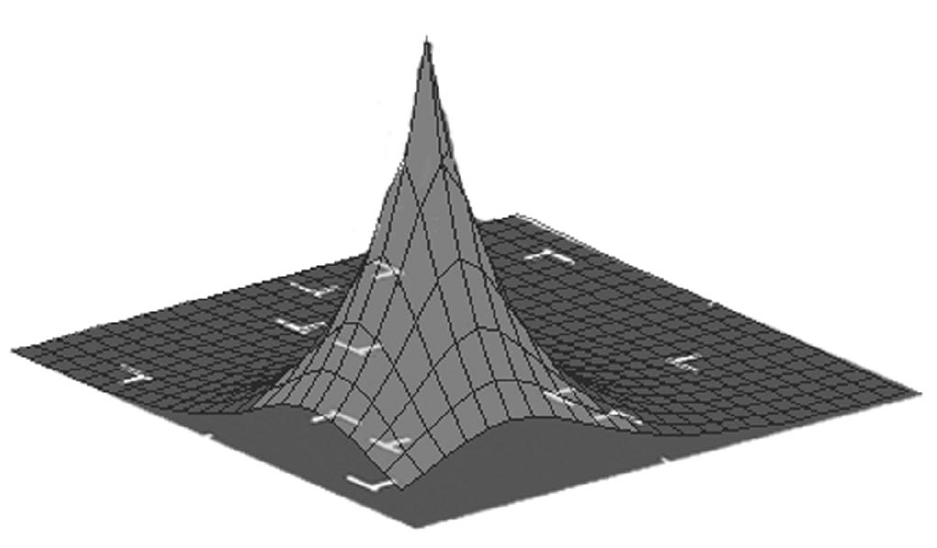
\includegraphics[width=0.6\linewidth]{fig_Brady2007_SC} 

}

\caption{Illustration of the spatial constraints on associative weight change in the Brady and Chun (2007) model}\label{fig:brady2007}
\end{figure}

Extensions of the Brady and Chun (2007) model have looked to extend and refine this associative framework for representing CC. Beesley et al. (2015) demonstrated the importance of local associative connections between input units, such that memory enocding of the configuration occurs irrespective of the associations that exist between the distractors and the target location. Similarly Beesley et al. (2016) developed a model that works with ``configural representations'' at the input layer and associates the entire configuration with the target location.

Importantly, all of these models have worked with two-dimensional representations of the search space, encoding the spatial information on an x/y coordinate space. This is because the vast majority of visual search research, and nearly all CC research, has presented stimuli across a two-dimensional coordinate space (i.e, a screen). Yet a great many (perhaps the vast majority) of real-world visual search tasks are performed on stimuli that exist in a three-dimensional coordinate space. From both an empirical and theoretical (model) perspective, it is important to determine the role that depth plays in the formation of representations of visual scenes and how that affects the CC of visual search.

It is well acknowledged that the visual system is highly attuned to the processing of depth information, and that the position of stimuli across depth planes can have important effects on visual search efficiency (e.g., McSorley \& Findlay, 2001; Nakayama \& Silverman, 1986). We focus here on the small group of studies that have explored the role of depth information in CC of visual search. Kawahara (2003) (Experiment 2A and 2B) used shutter glasses to render stereoscopic projections of stimuli across two depth planes, \emph{near} and \emph{far} from the viewer, with targets appearing equally across the two planes. Critically they were able to show a CC effect with this procedure, and when the distractors across the two planes were swapped in a final stage, the CC effect was reduced, though not completely abolished. The reduction of the effect demonstrates that the CC that had been established was reliant on the encoding of depth information, which was disrupted by the manipulation in the final stage.

Zang et al. (2017) have suggested that Kawahara's (2003) method of maintaining the position of the target during the switch of distractor depths may have disrupted the local associations between the target and distractors in terms of their two-dimensional representations (x/y). To test this, Zang et al.~(Experiment 1) subjected entire configurations to a depth reversal, including the depth of the target. Interestingly, they found that, in contrast to the findings of Kawahara (2003), the CC effect remained intact after the swap of depth planes. When the configurations of distractors were disrupted by switching the left and right sides (Experiment 2), the CC effect was significantly attenuated. Thus the results of Zang et al.'s (2017) Experiment 1 call into question how critical depth information is in the representations driving CC, at least to the extent that associations either do not appear to be forming across different depth planes, or are resistant to significant generalization decrements.

The current set of experiments further explore the role that depth plays in CC of visual search. The experiments use a virtual reality device to project the stimuli in stereoscopic 3D. This allows stimuli to be positioned across a wide field of view, with head movements required to process the visual display in full during the search process. Experiments 1a and 1b provide a simple demonstration of the CC effect in this novel procedure with targets placed relatively near to, or far from, the observer. In Experiment 2 we manipulate the validity of distractors at these different depths to explore the structure of the associative representations that form during visual search across three-dimensions.

\hypertarget{transparency-and-openness}{%
\subsection{Transparency and Openness}\label{transparency-and-openness}}

The data, analysis scripts, experimental materials, and the manuscript source files, are available at \href{https://github.com/tombeesley/CCVR}{github.com/tombeesley/CCVR}. We report our determination of sample sizes, the data exclusion criteria, and all of the manipulations. The analyses reported in this manuscript are computationally reproducible from the manuscript source files (using R v4.0.2), which are available at the github repository. The study design and analyses were not pre-registered.

\hypertarget{experiment-1}{%
\section{Experiment 1}\label{experiment-1}}

The current experiment aimed to demonstrate CC in the virtual reality procedure, while also providing a simple manipulation of the target depth. Stimuli in the experiment were positioned at one of two distances from the observer (hereafter `near' and `far' depths). On one half of all trials, repeated configurations were presented, in which all distractors across the two depths were positioned in set locations. On the other half of all trials, all distractors were arranged randomly. Orthogonal to this factor, targets were positioned at either near or far locations from the observer.\footnote{At the time of writing this manuscript we became aware of an experiment with a similar rationale and design published by Marek and Pollmann (2020)}

Vadillo et al. (2016) estimated an effect size of \emph{d\textsubscript{z}} = 1 in typical CC experiments. Given the novelty of the procedure, we took a cautionary approach by estimating a diminished effect size of \emph{d\textsubscript{z}} = 0.50. To achieve power of 0.90, with \(\alpha\) = 0.05, required a minimum sample of 44, which was achieved in Experiment 1 (Experiment 1a and 1b combined).

While running Experiment 1, it was found that there were occasions on which some participants struggled to complete a trial, and the experiment could not progress until the target had been accurately detected. To alleviate this issue, we added a timeout to the trial procedure, terminating the trial after 10 seconds. We also made some subtle changes to the target detection algorithm. We present the original procedure as Experiment 1a and the modified procedure as Experiment 1b. We assess the impact this modification made to the ease of target detection, and we include the ``sub-experiment'' factor in our analysis.

\hypertarget{experiment-1a}{%
\subsection{Experiment 1a}\label{experiment-1a}}

\hypertarget{method}{%
\subsection{Method}\label{method}}

\hypertarget{participants.}{%
\subsubsection{Participants.}\label{participants.}}

Twenty-five undergraduate psychology students (mean age = 19.44, SD = 2.02; 19 identified as male and 6 as female) from UNSW Sydney participated in the study in exchange for course credit (one participant failed to complete the task and their data were not analysed). Participants were required to have normal or corrected visual acuity. Participants wearing glasses (but not those wearing contact lenses) were excluded from this experiment due to constraints with the amount of space available in the virtual reality headset.

\hypertarget{materials.}{%
\subsubsection{Materials.}\label{materials.}}

An Oculus Rift CV1 headset (Oculus VR), connected to a PC with a NVIDIA GeForce GTX 970 graphics card, delivered the experiment in virtual reality. The Oculus Rift CV1 is a head-mounted display that utilises a stereoscopic OLED display with 2160 x 1200 resolution (1080 x 1200 per eye) at a refresh rate of 90 Hz. Within the headset, images on the computer undergo transformations through two convex hybrid Frensel lenses, warping images and extending the environment to a wide 110° field of view. The headset has a dial that adjusts the separation of the lenses to accommodate for the varying interpupillary distances across participants. Two external infrared tracking sensors were used to track the headset and position the user in 3D space. The experiment was programmed in the Unity engine, which created all the stimulus properties, controlled timing and recorded responses. All dimensions of the program were measured in ``Unity units.'' The spacebar was used for indicating the detection of the target.

The virtual reality environment depicted an empty room with grey walls where the viewer was situated in the middle of the room. The program allows objects to be placed on any of nine concave surfaces, which radiated from the observer at the origin point (see Figure \ref{fig:schematic}). Two of these surfaces were selected for the two depths (near and far) used in the task. Objects on each surface were approximately equidistant from the observer. Each surface represented an increment of 2 units from the observer.



\begin{figure}

{\centering 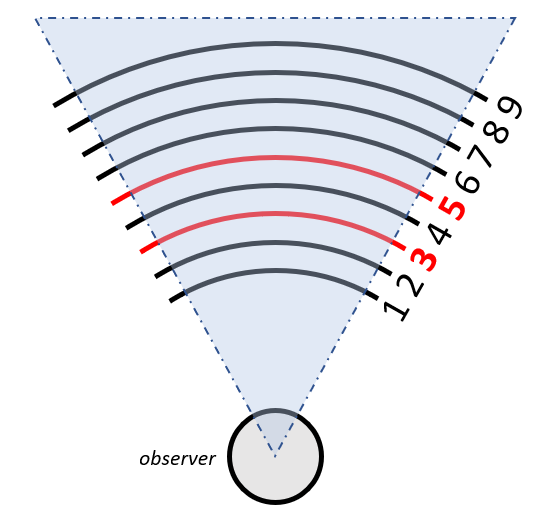
\includegraphics[width=0.6\linewidth]{VR_schematic} 

}

\caption{Schematic of the surface arrangement from a top-down perspective. The the choices for `near' (3) and `far' (5) surfaces are shown in red.}\label{fig:schematic}
\end{figure}

Object placement was restricted such that objects did not appear too far to the left or right of the viewer and too far above and below the viewer. As it was possible for stimuli to appear close to the observer, head movements were required to examine the configurations and to find the target. Surfaces 3 and 5 were chosen to provide an environment where stimuli were quite clearly positioned at different depths, while balancing the need for excessive head movements.

Each trial contained 16 cylinder-shaped distractor objects and one capsule-shaped (rounded) target. All stimuli were red and had a scale of 0.3 x 0.24 x 0.3 Unity units (x,y,z) regardless of depth. There were no constraints on the rotation on the x, y and z-axis for each target and distractor, but rotations were fixed for repeating configurations.

A semi-transparent blue disk was used in the practice phase, scaled at 0.18 x 0.18 x 0.001 Unity units (x,y,z), was presented in the middle of the participant's visual field (see Figure \ref{fig:task-example}). A white fixation disc was used throughout the task for refocusing, which was scaled at 1 x 1 x 0.001 Unity units(x,y,z).



\begin{figure}

{\centering 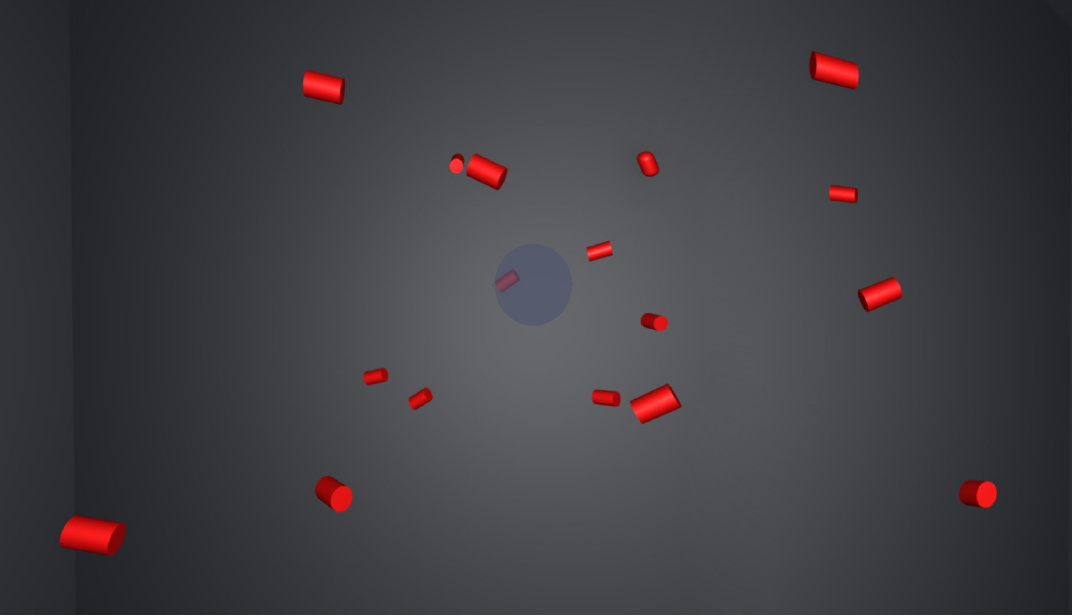
\includegraphics[width=0.6\linewidth]{fig_ExampleVR} 

}

\caption{Example stimulus arrangement. The central blue disc represents the centre of the participants view and was only present during the practice trials. The rounded target shape is located in the upper right quadrant.}\label{fig:task-example}
\end{figure}

\hypertarget{design.}{%
\subsubsection{Design.}\label{design.}}

A within-subjects design was used, with independent variables of \emph{configuration type} (repeated vs.~random), \emph{target-depth} (near vs.~far), and epoch (6 epochs, each comprising 5 blocks). The dependent variable of primary interest in all experiments was reaction time (head movements were recorded and those data are available at the \href{https://github.com/tombeesley/CCVR}{data repository}, but are not reported).

Each configuration comprised 16 cylinder-shaped distractors, which were equally distributed across the two surfaces, resulting in eight distractors per surface (Figure \ref{fig:task-example}). Within each surface, the eight distractors were distributed equally across the four quadrants of the x/y plane. The target was placed on one or other surface depending on the configuration set (see below), and within each set the target was equally frequent in each quadrant of the x/y plane. The same target locations were used in the repeating and random configuration types that had targets at the same depth. Two sets of configurations were repeated across the blocks of the experiment: \emph{Near-T-repeated} had targets on the near surface and repeating distractor configurations on both surfaces, while \emph{Far-T-repeated} had targets on the far surface and repeating distractor configurations on both surfaces. Two sets of ``random configurations'' were used in which distractors on the two surfaces were randomly arranged: \emph{Near-T-random} had targets on the near surface and \emph{Far-T-random} had targets on the far surface.

\hypertarget{procedure}{%
\subsubsection{Procedure}\label{procedure}}

Participants were given 10 practice trials to familiarize themselves with the task. This provided participants with a guide as to how they should direct their head position towards the centre of the target object, prior to responding with the spacebar. Participants were told to search for a ``pill-shaped target'' and to press the spacebar once the central blue circle region was over the target object. This provided a guide to how the program would register accurate target detection. The blue circle was used for training only and not presented in the main phase of the experiment. After a successful detection of the target, the white fixation circle appeared. The program detected the gaze on this fixation circle before initiating the next trial.

The main task consisted of 480 trials, divided into 30 blocks (16 trials per block). Each block contained four trials from each of four different configuration sets. Within each set, and within each block, targets were equally distributed across the four quadrants of the x/y plane. The order of trials within each block was randomised, with the constraint that the target could not occupy the same location across consecutive trials. Participants were given breaks every 160 trials (at the end of every 10 blocks) and breaks lasted until participants wished to resume.

Reaction times were measured in milliseconds (ms) from the beginning of a trial to an accepted target detection response for each trial. Any rejected target detection responses - those that were made when the headset was not oriented accurately on the target - were recorded and used to determine the difficulty of target detection on any given trial.

\hypertarget{experiment-1b}{%
\subsection{Experiment 1b}\label{experiment-1b}}

\hypertarget{method-1}{%
\subsection{Method}\label{method-1}}

\hypertarget{participants.-1}{%
\subsubsection{Participants.}\label{participants.-1}}

Twenty participants (mean age = 23.65, SD = 5.39; 5 participants identified as male and 15 as female) took part in the study in exchange for AUS\$15. All other aspects of participant recruitment, exclusions and requirements were identical to Experiment 1a.

\hypertarget{materials-design-and-procedure.}{%
\subsubsection{Materials, Design, and Procedure.}\label{materials-design-and-procedure.}}

Experiment 1b employed some minor alterations to the materials and procedure. Sixteen practice trials were used instead of 10. Breaks were given every 64 trials (every four blocks) compared to every 160 trials in Experiment 1A. In an attempt to combat issues with object occlusion and poor target detection rates, a timeout was given (the word ``TIMEOUT'' appeared) after 10 seconds of the trial. Experiment 1b also used an updated algorithm controlling the registration of the participants view over targets in an attempt to improve valid target detection.

\hypertarget{results}{%
\subsection{Results}\label{results}}

Since Experiment 1B used a timeout of 10 seconds, we imposed the same cutoff for our analysis of reaction times in Experiment 1A. Trials which led to timeouts and trials that had more than two response attempts were removed (i.e., up to 2 spacebar responses were allowed). Following this, RTs greater or less than 2.5 SDs from the participant mean RT were removed. On average, these data processing steps led to the removal of 13.10\% of trials. Mean RTs for each participant were computed and the mean across the sample was 2310 ms (SD = 388). No participants were identified as outliers in terms of their mean RT.

Two participants had an unusually high proportion of trials removed (greater than 2.5 SDs of the mean proportion of trials removed), and we excluded these two participants from further analysis. We next examined the proportion of trials contributing to the analysis across trials with targets at the two different depths. Our concern here was that if targets were harder to detect at the more distant depth, which would result in a greater level of exclusion for those trials, that this may bias the size of the contextual cuing for trials with targets at different depths. We identified 6 participants (4 from Experiment 1a and 2 from Experiment 1b) that had a high discrepancy in the proportion of excluded trials across the factor of target depth (greater than 15\% difference in the proportion of trials excluded) and we excluded these participants from further analysis. The final proportion of trials contributing to the analysis in Experiment 1a was 93.9\% and 88.2\% for near and far targets, respectively, and in Experiment 1b was 87.9\% and 88.4\% for near and far targets, respectively.

Within-subject error bars were computed by a process of normalising the RT data for the sample (Cousineau, 2005). Figure \ref{fig:Exp1-RT-figure} shows the RT data across the 6 epochs, plotted separately for the data from Experiment 1a and Experiment 1b. RTs decreased with practice on the task, and were shorter for repeated configurations than for random configurations. There was also a clear target location effect, with responses being much slower when the target was located on the near surface compared to the far surface.



\begin{figure}

{\centering 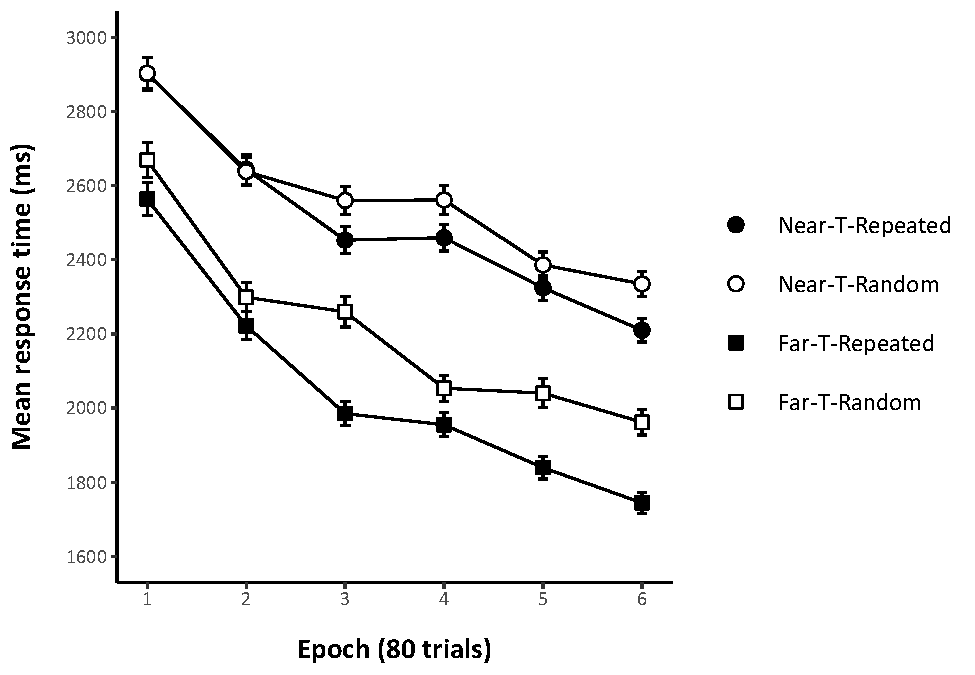
\includegraphics[width=1\linewidth]{CCVR_manuscript_files/figure-latex/Exp1-RT-figure-1} 

}

\caption{RT data for Experiment 1A and 1B.}\label{fig:Exp1-RT-figure}
\end{figure}

These data were subjected to a four-way repeated measures ANOVA, with a between-subject factor of \emph{sub-experiment} (1a vs.~1b), and within-subject factors of \emph{configuration type} (repeated vs.~random), \emph{target-depth} (near vs.~far) and \emph{epoch} (1 to 6). Where Mauchly's test of sphericity revealed violations, Greenhouse-Geisser corrections were made. There was no main effect of \emph{sub-experiment}, \emph{F}(1, 35) = 0.07, \emph{p} = .800, \(\eta^2_p\) \textless{} .01 and the only significant interaction effect involving \emph{sub-experiment} was the \emph{sub-experiment} by \emph{configuration type} by \emph{epoch} interaction, \emph{F}(3.78, 132.16) = 2.76, \emph{p} = .033, \(\eta^2_p\) = .07, suggesting that the contextual cuing effect may have emerged at slightly different rates in the two procedures{[}FOOTNOTE HERE{]}.

There was a main effect of \emph{configuration type}, \emph{F}(1, 35) = 15.58, \emph{p} \textless{} .001, \(\eta^2_p\) = .31, with response times for repeated configurations (2220.6 ms, SD = 379) faster than those for random configurations (2323.7 ms, SD = 380). There was a main effect of \emph{target-depth}, \emph{F}(1, 35) = 80.12, \emph{p} \textless{} .001, \(\eta^2_p\) = .70, with response times for far targets (2076.6 ms, SD = 384.5) faster than those for near targets (2467.8 ms, SD = 402.8). There was also a main effect of \emph{epoch}, \emph{F}(3.50, 122.46) = 69.44, \emph{p} \textless{} .001, \(\eta^2_p\) = .66 with response times decreasing across the experiment. The \emph{configuration type} by \emph{target-depth} interaction was not significant, \emph{F}(1, 35) = 3.23, \emph{p} = .081, \(\eta^2_p\) = .08. The \emph{configuration type} by \emph{epoch} interaction was significant, \emph{F}(3.78, 132.16) = 4.73, \emph{p} = .002, \(\eta^2_p\) = .12, as was the \emph{target-depth by epoch} interaction, \emph{F}(5, 175) = 3.84, \emph{p} = .003, \(\eta^2_p\) = .10, suggesting that the RT decrease was more pronounced for configurations with distal targets. There were no other significant interaction effects.

The overall CC effect (the main effect of \emph{configuration type} from the ANOVA) resulted in a Cohen's \emph{d\textsubscript{z}} = 0.66, with 78\% of participants showing a positive CC effect. The CC effect was present in both configurations with near targets, \emph{t}(36) = 2.08, \emph{p} = .045, \emph{d\textsubscript{z}} = 0.34, and those with far targets, \emph{t}(36) = 3.76, \emph{p} \textless{} .001, \emph{d\textsubscript{z}} = 0.62.

\hypertarget{discussion}{%
\subsection{Discussion}\label{discussion}}

Experiment 1 established a VR procedure for observing a CC effect, which resulted in a moderately large effect size of \emph{d\textsubscript{z}} = 0.66. This is somewhat weaker than the CC effect seen in some standard 2D implementations of the task. Interestingly the effect was modulated by the depth of the target: those configurations that were paired with a target on the far surface were learnt about more readily than those paired with targets on the near surface. This was coupled with an overall target-depth effect and it's possible that these two effects are related. When targets are positioned close to the observer, they are harder to detect, and this will lead to slower and possibly more variable search processes. In turn, a more random process of sampling the visual scene might lead to weaker distractor-target associations, resulting in weaker CC.

Marek and Pollmann (2020) have previously shown evidence of a CC effect in a virtual reality procedure. Like in our task, participants experienced targets appearing on either a near surface or a far surface. In their task, and unlike in our results, participants took longer to respond to targets on the far surface compared to the near surface. This is likely to be because, in Marek and Pollmann's (2020) task, the targets on the far surface were placed outside of the immediate field of view, and hence head movements were needed to locate the targets on the far surface. In contrast, in Experiment 1 it was the targets on the near surface that could be placed outside of the initial field of view, whilst the targets on the far surface had a far greater chance of being contained within the initial field of view. Taken together, the two experiments (Experiment 1 and Marek and Pollmann (2020)) show, somewhat unsurprisingly, that the presence of the target within the initial field of view is critical to the speed of target detection.

\hypertarget{experiment-2}{%
\section{Experiment 2}\label{experiment-2}}

While Experiment 1 showed that CC varies as a function of the placement of the target, it is unclear what role depth plays in the formation of associations within repeating configurations. For example, it could be that associations only form between distractors and targets co-occurring on the same surface. Experiment 2 addresses this question directly by selectively pairing distractor configurations at one of the two depths, with targets that are placed at one of the two depths. As such, for each repeating configuration of distractors, half of the distractors were repeated across presentations and the other half were randomly arranged. For some participants, the distractors on the proximal surface to the target repeated, while for other participants the distractors on the distal surface to the target repeated. By also manipulating the target depth (relative to the observer) across configurations, this produced orthogonal factors of target depth, and repeated distractor depth.

This design allowed us to test the strength of associations forming between distractors and targets (i.e., to test whether CC is greater when repeating distractors are positioned close to the target or far away from the target). We decided to manipulate the relationship between the repeating distractors and the target on a between-subjects basis in order to reduce the total number of configurations participants were exposed to (given the clear limitations on learning in standard CC designs, cf. Smyth and Shanks (2008)). Thus participants were exposed to eight repeated configurations: four with the target placed on the near surface, and four with the target on the far surface (within each set, the target was placed once within each quadrant).

In order to maximise the learning of these distractor-target associations (in what were quite stochastic configurations), we exposed participants to repeated configurations in ``training'' blocks, without the presentation of any random configuration trials. In order to then test for CC, we presented the entirely random configurations alone in ``test'' blocks. If CC had occurred during training, then we would expect to see increases in RT on the test blocks. By ensuring random configurations shared the same target positions, we were able to examine the CC effect for different types of configurations. For example, performance on the repeated configurations with near targets can be directly compared to the performance on the random configurations with those same near targets.

We also included an ``awareness test'' at the end of the experiment. Participants were presented with repeated configurations from the main experiment and newly generated configurations. On each presentation, the target was replaced with a distractor and participants were asked to identify (guess) which distractor had replaced the target.

\hypertarget{method-2}{%
\subsection{Method}\label{method-2}}

\hypertarget{participants.-2}{%
\subsubsection{Participants.}\label{participants.-2}}

Sixty-eight participants (mean age = 19.32, SD = 2.33; 20 participants identified as male and 48 as female) from UNSW Sydney took part in the study in exchange for AUS\$15. Participants were randomly allocated to one of the two target-distractor contingency conditions, ``proximal'' and ``distal.'' 34 participants were allocated to each condition. One participant from each condition was excluded from further analysis on the basis of their mean RT (see below).

All other aspects of participant recruitment, exclusions and requirements were identical to Experiment 1a and 1b.

\hypertarget{materials-design-and-procedure.-1}{%
\subsubsection{Materials, Design, and Procedure.}\label{materials-design-and-procedure.-1}}

The materials used were the same as those used in Experiment 1b, with the exception that surfaces 3 and 6 were used to accentuate the differences in depth (see Figure \ref{fig:schematic})

A mixed-model design was used, with a between-subject factor of \emph{target-distractor contingency} (proximal vs.~distal), and within-subject factors of \emph{configuration type} (repeated vs.~random), \emph{target-depth} (near vs.~far) and \emph{epoch} (31 epochs, each comprising 2 blocks).

Configurations were created in the same manner as for Experiment 1a and 1b, except that the sets of repeated configurations contained repeating distractors on only one surface. Each presentation of one of these repeating configurations contained a novel random configuration of distractors on the ``non-repeating surface.''

The procedure was the same as that used in Experiment 1b, with the exception that random configurations were only presented in epochs 9, 10, 19, 20, 29, and 30, and repeated configurations were not presented in these 6 epochs.

At the end of the task participants were given a ``generation awareness test.'' Two blocks of 16 trials were given, which each included the 8 repeating configurations from the main task, and 8 new repeating configurations that had been created in an identical manner (i.e., these new configurations were repeated in the second block). On each trial, the target object was replaced by a distractor object. Participants had to centre their view over the distractor they thought was most likely to be the target and press the spacebar. The program computed the discrepancy between the true target and the centre of the visual field, computing this error in two-dimensional space (x and y). This error measure (in unity units) acted as the dependent variable for the awareness task. A smaller error score on repeated compared to random configurations would indicate a level of awareness of where the target was positioned in repeating configurations.

\hypertarget{results-1}{%
\subsection{Results}\label{results-1}}

Trials were excluded on the same basis as in Experiment 1a and 1b. On average, this led to the removal of 9.60\% of trials.

Mean RTs for each participant were computed and the mean across the sample was 2190 ms (SD = 345). As detailed above, two participants were excluded as outliers, as their mean RT was more than 2.5 SDs higher than the mean of the sample.

Figure \ref{fig:Exp2-RT-figure} shows the RT data across the 31 epochs. RTs decrease with practice on the task, and are shorter for repeated configurations than for random configurations. Like in Experiment 1a and 1b, there is a clear target location effect, with responses being much slower when the target was located on the near surface compared to when it was on the far surface.



\begin{figure}

{\centering 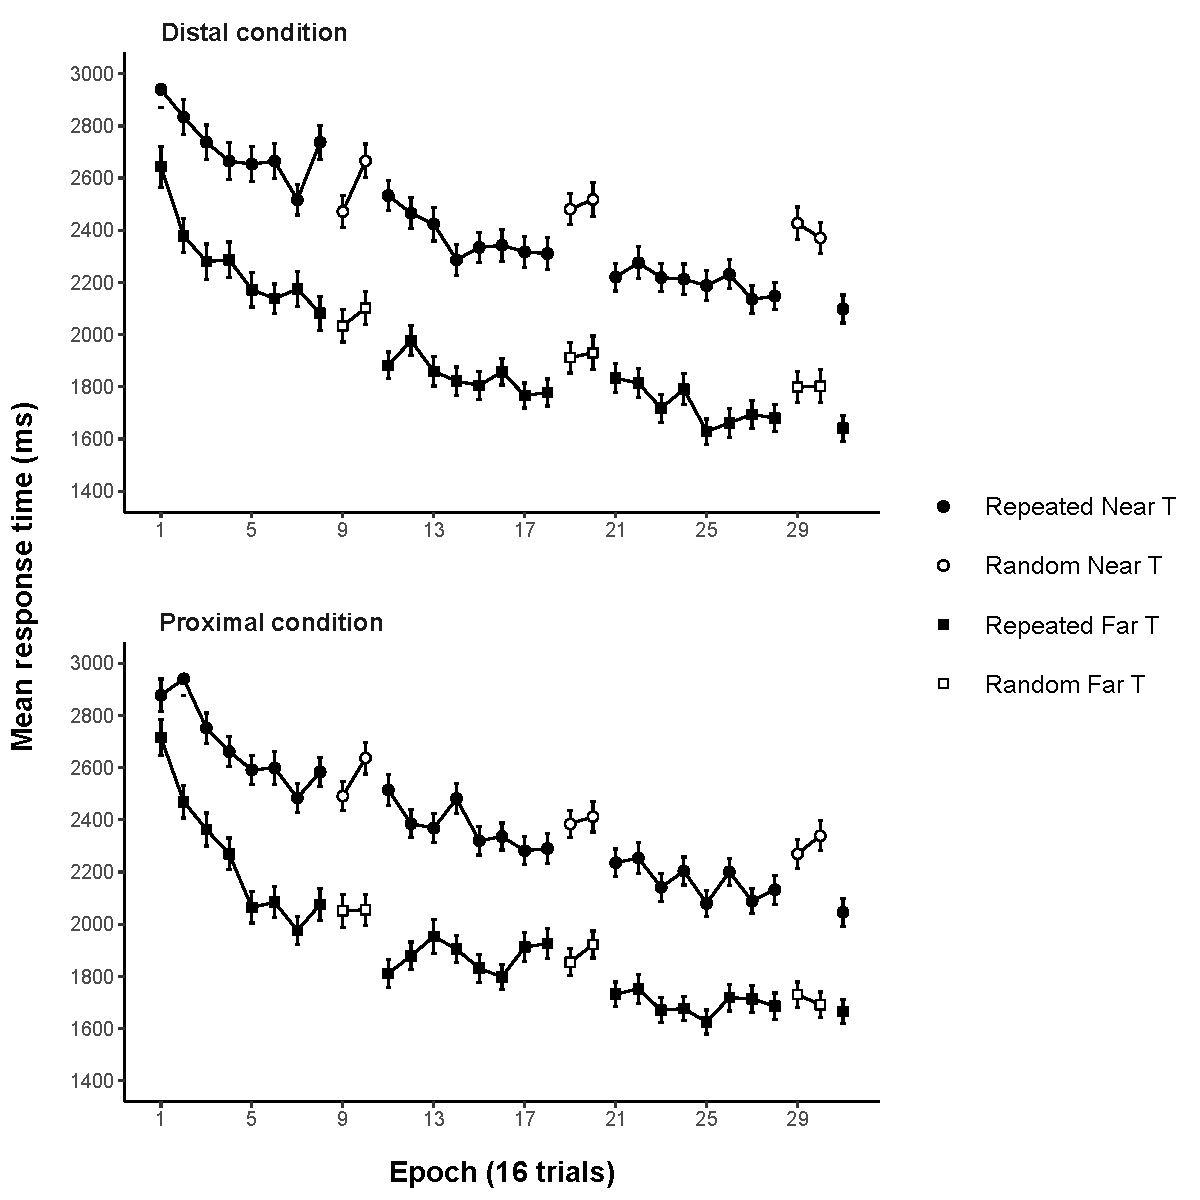
\includegraphics{CCVR_manuscript_files/figure-latex/Exp2-RT-figure-1} 

}

\caption{RT data for Experiment 2.}\label{fig:Exp2-RT-figure}
\end{figure}

Learning effects under each condition were calculated by comparing RTs for those epochs containing random configurations (9, 10, 19, 20, 29, and 30) with the adjacent epochs containing repeated configurations (8, 11, 18, 21, 28, 31). The data from these three ``test periods'' are plotted in Figure \ref{fig:Exp2-test-figure}.



\begin{figure}

{\centering 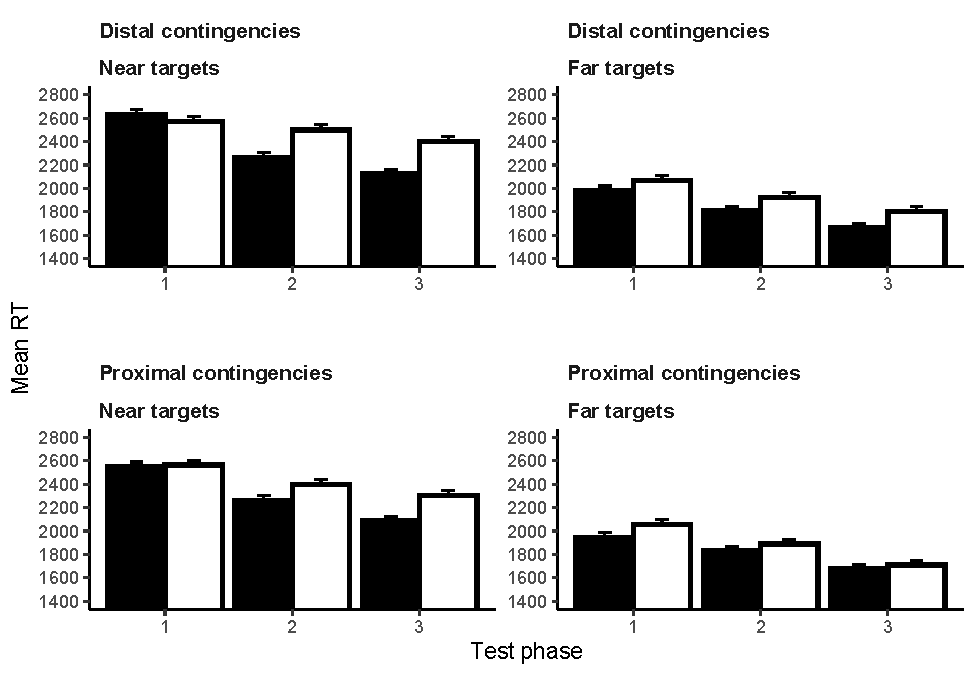
\includegraphics[width=1\linewidth]{CCVR_manuscript_files/figure-latex/Exp2-test-figure-1} 

}

\caption{RT data from the ``test blocks'' of Experiment 2.}\label{fig:Exp2-test-figure}
\end{figure}

The data were subjected to a four-way mixed-model ANOVA with a between-subject factor of \emph{target-distractor contingency} (proximal vs.~distal), and within-subject factors of \emph{configuration type} (repeated vs.~random), \emph{target-depth} (near vs.~far) and \emph{test} (test 1, 2, or 3). Where Mauchly's test of sphericity revealed violations, Greenhouse-Geisser corrections were made. There was a main effect of \emph{configuration type}, \emph{F}(1, 64) = 36.31, \emph{p} \textless{} .001, \(\eta^2_p\) = .36, with response times for repeated configurations (2058.9 ms, SD = 307) faster than those for random configurations (2180.4 ms, SD = 299.9). There was also a main effect of \emph{target-depth}, \emph{F}(1, 64) = 204.73, \emph{p} \textless{} .001, \(\eta^2_p\) = .76, with response times for far targets (1859.2 ms, SD = 325.2) faster than those for near targets (2380.2 ms, SD = 328.8). The main effect of \emph{test} was also significant, \emph{F}(2, 128) = 69.95, \emph{p} \textless{} .001, \(\eta^2_p\) = .52 with response times decreasing across the three tests (Test 1: 2291.8 ms, SD = 335.7; Test 2: 2103.4 ms, SD = 318.9; Test 3: 1963.9 ms, SD = 303.5). The main effect of \emph{target-distractor contingency} was not significant, \emph{F}(1, 64) = 0.21, \emph{p} = .646, \(\eta^2_p\) \textless{} .01.

There was a significant interaction between \emph{configuration type} and \emph{test}, \emph{F}(2, 128) = 6.11, \emph{p} = .003, \(\eta^2_p\) = .09, indicating that the difference in response times between repeated and random configurations increased across the three tests. There was no significant \emph{configuration type} by \emph{target-depth} interaction, \emph{F}(1, 64) = 1.39, \emph{p} = .243, \(\eta^2_p\) = .02, however there was a significant three-way interaction between \emph{configuration type}, \emph{target-depth}, and \emph{test}, \emph{F}(2, 128) = 8.89, \emph{p} \textless{} .001, \(\eta^2_p\) = .12. To explore this in more detail, we calculated a CC score, subtracting the response times for repeated configurations from those for random configurations, and plotted this score across the three tests as a factor of target-depth. These data are shown in Figure \ref{fig:Exp2-CC-figure}. As can be seen, the CC effect for configurations with targets on the far surface is fairly consistent across the three tests, whereas the CC effect for configurations with targets on the near surface is initially weaker, but is then stronger across tests 2 and 3. Post-hoc t-tests compared differences in CC for configurations with near and far targets at each of the three tests, revealing that the CC effect was different in Test 1, \emph{t}(65) = -2.13, \emph{p} = .037, \emph{d\textsubscript{z}} = -0.26, and Test 3, \emph{t}(65) = 3.02, \emph{p} = .004, \emph{d\textsubscript{z}} = 0.37, but not Test 2, \emph{t}(65) = 1.73, \emph{p} = .088, \emph{d\textsubscript{z}} = 0.21. No other interaction effects were significant.



\begin{figure}

{\centering 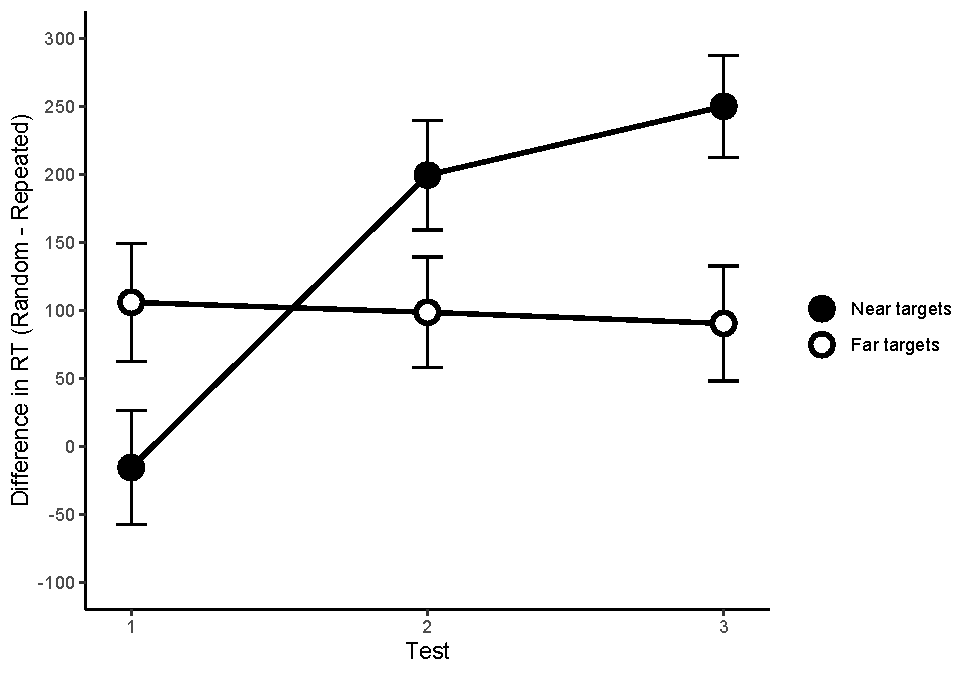
\includegraphics[width=1\linewidth]{CCVR_manuscript_files/figure-latex/Exp2-CC-figure-1} 

}

\caption{CC effect across tests in Experiment 2, as a function of target-depth.}\label{fig:Exp2-CC-figure}
\end{figure}

\hypertarget{analysing-the-egocentricity-of-learning}{%
\subsubsection{Analysing the egocentricity of learning}\label{analysing-the-egocentricity-of-learning}}

So far our analysis has focused on the \emph{allocentric} nature of the contingencies: whether the position of the repeating distractors in respect of the target-depth affects the CC that develops. However, our manipulation of the distractor contingencies, with only one surface containing repeated distractors (and the other random distractors) means that we can also assess the CC effect with respect to the position of the observer. To do this, we recoded the factors of distractor-target contingency and target depth as a single factor of egocentricity: egocentric-near (proximal contingencies with near targets; distal contingencies with far targets) or egocentric-far (proximal contingencies with far targets; distal contingencies with near targets). These data are presented in Figure \ref{fig:Exp2-ego-figure}.



\begin{figure}

{\centering 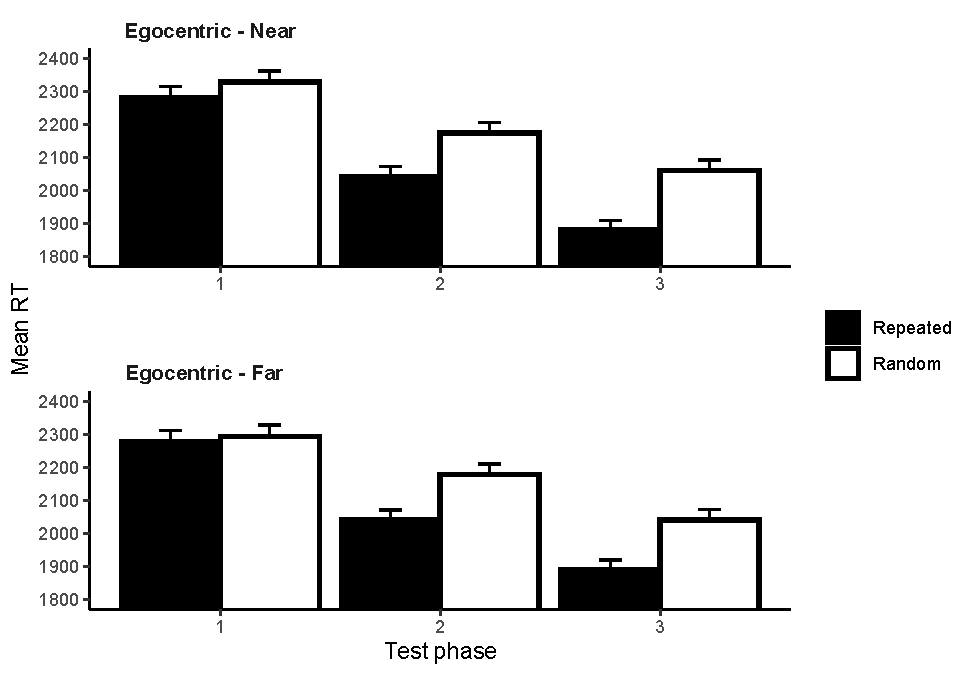
\includegraphics[width=1\linewidth]{CCVR_manuscript_files/figure-latex/Exp2-ego-figure-1} 

}

\caption{RTs across the tests in Experiment 2, as a function of egocentricity of the repeated configurations (near to the observer or far from the observer).}\label{fig:Exp2-ego-figure}
\end{figure}

These data were subjected to a three-way repeated-measures ANOVA with factors of \emph{egocentricity}, \emph{configuration type} and \emph{test}, which found no main effect of egocentricity, and egocentricity did not interact with the other factors (\emph{F}s \textless{} 1). To confirm the CC effect in both conditions, separate ANOVAs were run on the near and far egocentric conditions. This revealed main effects of configuration type and test in both conditions (\emph{F}s \textgreater{} 17). The interaction between configuration type and test was significant in the far condition, \emph{F}(2, 130) = 3.27, \emph{p} = .041, \(\eta^2_p\) = .05, but not in the near condition, \emph{F}(2, 130) = 3.03, \emph{p} = .052, \(\eta^2_p\) = .04.

\hypertarget{awareness-test}{%
\subsubsection{Awareness test}\label{awareness-test}}

For the awareness test, participants error scores (Euclidean distance on the x/y plane, between the correct target position and central head position in ``Unity units'') on configurations with far targets was 4.5 (SD = 2.73) for repeated configurations, and 4.53 (SD = 2.73) for random configurations, while for near targets it was 3.14 (SD = 1.8) for repeated configurations, and 3.35 (SD = 1.77) for random configurations. These data were subjected to a two-way ANOVA with factors of \emph{configuration} and \emph{target-depth}, which revealed a main effect of target-depth \emph{F}(1, 65) = 153.15, \emph{p} \textless{} .001, \(\eta^2_p\) = .70,\footnote{The main effect of target-depth is due to the relative distances between the objects on the near surface being shorter than those on the far surface. Therefore any given decision made will be more likely to be closer to the actual target position for near surface targets} but no main effect of configuration, \emph{F}(1, 65) = 1.40, \emph{p} = .241, \(\eta^2_p\) = .02 and no interaction, \emph{F}(1, 65) = 0.56, \emph{p} = .455, \(\eta^2_p\) \textless{} .01. A Bayesian ANOVA revealed a Bayes Factor of 0.20 for the model containing only the configuration factor, suggesting reasonable support for the null model.

\hypertarget{discussion-1}{%
\subsection{Discussion}\label{discussion-1}}

Experiment 2 sought to examine the associative learning occurring between distractors and targets across different depths during visual search. For all participants, targets appeared on either the near or far surface equally often, and half of the distractors were repeated (and so could be learnt in relation to the target), while the other half of the distractors on each trial were randomly arranged. For half of the participants, the repeating distractors were those that were proximal to the target (same surface), and for the other half of participants the repeating distractors were those that were distal to the target (different surface). We found that the proximity of the repeating distractors to the target did not affect the size of the CC effect. As in Experiment 1, the target-depth appears to play a more important role in determining visual search and CC. As was the case in Experiment 1, targets that appear nearer to the observer were harder to detect (slower RTs). However, unlike in Experiment 1, this eventually led to a larger CC effect for distractors paired with those near targets. This was borne out in the three-way interaction effect between configuration type, target-depth, and test, with the final test phase revealing a larger CC effect for configurations with targets on the near surface compared to the CC effect for those configurations with targets on the far surface.

We also examined any potential effect of the ego-centricity of repeating distractors on CC, by coding the configurations as either containing repeating distractors that appeared near or far from the observer. This confirmed that ego-centricity did not affect CC and that both levels of ego-centricity resulted in CC.

An awareness test, in which participants had to indicate the location of an absent target, revealed that participants were as accurate for new configurations as they were for those that they had experienced in the main task. The procedure involved the presentation of each configuration twice (32 trials in total), which goes some way towards alleviating issues of test sensitivity, though we acknowledge that a test involving more trials would be beneficial here (c.f. Smyth \& Shanks, 2008). As such, while our awareness test failed to find any evidence of conscious awareness of the repeating configurations, we acknowledge the issues with drawing such conclusions (see Vadillo et al., 2016, 2021).

\hypertarget{general-discussion}{%
\section{General Discussion}\label{general-discussion}}

Two experiments sought to establish a CC effect within a three-dimensional virtual reality procedure. Experiment 1 established a moderate effect of CC (Cohen's \emph{d\textsubscript{z}} = 0.66) and we observed a CC effect for both configurations with targets near to the observer, and those with targets more distant from the observer. Experiment 2 sought to examine the learning of proximal and distal contingencies within the repeating configurations, by selectively pairing the target with repeated configurations on the same surface, or the alternative surface. While we found a robust CC effect overall (0.74), there was no effect of the position of the repeated distractors on the size of the CC effect. These data overwhelmingly suggest that where contingencies exist within the repeating configurations, learning will occur readily for those target-distractor contingencies.

The placement of the target at different depths within three-dimensional space had a noticeable effect on the efficiency of visual search: having a target closer to the observer made search more difficult. Interestingly, there was some evidence in our data that the target placement also modulates the extent to which a CC effect develops. In Experiment 1 we found that the CC effect was stronger when repeated configurations were paired with targets on the far surface (those receiving faster responses) compared to the CC effect for repeated configurations paired with targets on the near surface (those receiving slower responses). However, Experiment 2 failed to fully replicate this effect. Instead, we found this advantage was observed only in the very first part of the experiment (Test 1), whereas later in the experiment this advantage had reversed (Test 3), with stronger CC effects observed for those configurations with targets on the near surface.

There were several differences between the two studies that could explain this pattern of findings. It's notable that the two training procedures were not equivalent in the extent to which they exposed participants to repeated configurations of the distractors. In Experiment 2 we trained repeated configurations alone for most of the experiment, with random configurations restricted to discrete test blocks. This would likely have led to an enhancement of contingency learning, but this would be offset to some degree by the more stochastic nature of the repeated configurations, with only half of the distractors in each repeated configuration predictive of the target in Experiment 2. In fact, the overall CC effect at the end of Experiment 2 (Test 3) was 170 ms, which was comparable to the effect seen in the final epoch of Experiment 1 of 182 ms. Inspection of the RT data from Experiment 2 (Figure \ref{fig:Exp2-RT-figure}), however, shows that RTs may have reached a floor in the conditions with far targets in the latter stages of the experiment. In comparison, inspection of the RT data from Experiment 1 (Figure \ref{fig:Exp1-RT-figure}) reveals no such floor effect in the RTs. A tentative conclusion may be that when RTs were not approaching, or at, floor in Experiment 2, the CC effect for far targets outstripped that for near targets (Test 1), but that the CC effect for far targets was suppressed in the later stages of Experiment 2 when RTs reached floor in the far target condition. In a related unpublished experiment from our lab, participants were trained with complete configurations of repeated distractors with both far and near targets (in a similar manner to Experiment 1). Here we observed no significant difference between the CC effect in near and far targets, but it was numerically larger for those with far targets. In addition to the data from our lab, Marek and Pollmann (2020) found no difference in the CC effect between configurations paired with near and far targets, with substantial support for the null hypothesis.

The finding that depth relationships did not modulate the size of the CC effect in Experiment 2 is consistent with the results of Zang et al. (2017), where it was observed that after successful CC had been established, switching the distractors (and target) between front and back planes resulted in a maintenance of CC. Taken together, these data suggest that CC relies predominantly (and possibly exclusively) on the formation of associations within a two-dimensional representation of space. Our analysis of the ego-centricity of the contingencies illustrates this feature: distractors occurring near to the participant were learnt as readily as distractors far from the participant.

In this sense, the associative framework put forward by Brady and Chun (2007; see also Beesley et al., 2016) to account for data from two-dimensional CC tasks would not require a major revision to allow for the encoding of depth information. As it stands, the three-dimensional configuration of distractors could be recoded as a two-dimensional configuration, ignoring the distance in depth between distractors and between distractors and the target.

Two caveats should be made to this conclusion. Firstly, Kawahara (2003) showed that reversing the depth of two surfaces within previously learnt configurations can produce a disruption in CC, but in the case of their experiment (in comparison to Zang et al., 2017), the target-depth was maintained across these reversals, and it is therefore likely that the two-dimensional relationships between distractors and targets were also disrupted. As such, this attenuation of the CC effect would be expected according to models encoding only two-dimensional representations of the configurations. The second caveat is that we observed a strong effect of target location on the efficiency of visual search, with longer search times on targets closer to the observer compared to targets appearing further away. Prima facie, this result would seem to necessitate the encoding of depth within the model to account for such effects on visual search. In addition, we have noted that this target depth effect appears to modulate the CC effect, though these results are less clear. It is possible, however, that harder visual searches simply result in weaker CC, irrespective of any manipulation of depth.

Our tasks demonstrate the great potential virtual reality procedures have for expanding the range of manipulations that can be achieved in CC (see also Marek \& Pollmann, 2020), and therefore advancing our understanding of the cognitive and perceptual processes responsible for learning in visual search. Future work will provide further tests of whether the ubiquitous CC effects across depth that we have observed withstand manipulations of distractor positions, providing further data to understand the discrepancy in findings between the current data, those of Zang et al. (2017) and those of Kawahara (2003). This in turn will provide key data to revise our models of CC.

\newpage

\hypertarget{references}{%
\section*{References}\label{references}}
\addcontentsline{toc}{section}{References}

\hypertarget{refs}{}
\begin{CSLReferences}{1}{0}
\leavevmode\hypertarget{ref-beesley2018}{}%
Beesley, T., Hanafi, G., Vadillo, M. A., Shanks, David. R., \& Livesey, E. J. (2018). Overt attention in contextual cuing of visual search is driven by the attentional set, but not by the predictiveness of distractors. \emph{Journal of Experimental Psychology: Learning, Memory, and Cognition}, \emph{44}(5), 707--721. \url{https://doi.org/10.1037/xlm0000467}

\leavevmode\hypertarget{ref-beesley2015b}{}%
Beesley, T., Vadillo, M. A., Pearson, D., \& Shanks, D. R. (2015). Pre-exposure of repeated search configurations facilitates subsequent contextual cuing of visual search. \emph{Journal of Experimental Psychology: Learning, Memory, and Cognition}, \emph{41}(2), 348--362. \url{https://doi.org/10.1037/xlm0000033}

\leavevmode\hypertarget{ref-beesley2016}{}%
Beesley, T., Vadillo, M. A., Pearson, D., \& Shanks, D. R. (2016). Configural learning in contextual cuing of visual search. \emph{Journal of Experimental Psychology: Human Perception and Performance}, \emph{42}(8), 1173--1185. \url{https://doi.org/10.1037/xhp0000185}

\leavevmode\hypertarget{ref-brady2007}{}%
Brady, T. F., \& Chun, M. M. (2007). Spatial constraints on learning in visual search: {Modeling} contextual cuing. \emph{Journal of Experimental Psychology: Human Perception and Performance}, \emph{33}(4), 798--815. \url{https://doi.org/10.1037/0096-1523.33.4.798}

\leavevmode\hypertarget{ref-chun1998}{}%
Chun, M. M., \& Jiang, Y. (1998). Contextual {Cueing}: {Implicit Learning} and {Memory} of {Visual Context Guides Spatial Attention}. \emph{Cognitive Psychology}, \emph{36}(1), 28--71. \url{https://doi.org/10.1006/cogp.1998.0681}

\leavevmode\hypertarget{ref-colagiuri2016}{}%
Colagiuri, B., \& Livesey, E. J. (2016). Contextual cuing as a form of nonconscious learning: {Theoretical} and empirical analysis in large and very large samples. \emph{Psychonomic Bulletin \& Review}, \emph{23}(6), 1996--2009. \url{https://doi.org/10.3758/s13423-016-1063-0}

\leavevmode\hypertarget{ref-cousineau2005}{}%
Cousineau, D. (2005). Confidence intervals in within-subject designs: {A} simpler solution to {Loftus} and {Masson}'s method. \emph{Tutorials in Quantitative Methods for Psychology}, \emph{1}(1), 42--45. \url{https://doi.org/10.20982/tqmp.01.1.p042}

\leavevmode\hypertarget{ref-kawahara2003}{}%
Kawahara, J. (2003). Contextual cueing in {3D} layouts defined by binocular disparity. \emph{Visual Cognition}, \emph{10}(7), 837--852. \url{https://doi.org/10.1080/13506280344000103}

\leavevmode\hypertarget{ref-marek2020}{}%
Marek, N., \& Pollmann, S. (2020). Contextual-{Cueing} beyond the {Initial Field} of {View}-{A Virtual Reality Experiment}. \emph{Brain Sciences}, \emph{10}(7). \url{https://doi.org/10.3390/brainsci10070446}

\leavevmode\hypertarget{ref-mcsorley2001}{}%
McSorley, E., \& Findlay, J. M. (2001). Visual search in depth. \emph{Vision Research}, \emph{41}(25-26), 3487--3496. \url{https://doi.org/10.1016/s0042-6989(01)00197-3}

\leavevmode\hypertarget{ref-nakayama1986}{}%
Nakayama, K., \& Silverman, G. H. (1986). Serial and parallel processing of visual feature conjunctions. \emph{Nature}, \emph{320}(6059), 264--265. \url{https://doi.org/10.1038/320264a0}

\leavevmode\hypertarget{ref-olson2002}{}%
Olson, I. R., \& Chun, M. M. (2002). Perceptual constraints on implicit learning of spatial context. \emph{Visual Cognition}, \emph{9}(3), 273--302. \url{https://doi.org/10.1080/13506280042000162}

\leavevmode\hypertarget{ref-smyth2008}{}%
Smyth, A. C., \& Shanks, D. R. (2008). Awareness in contextual cuing with extended and concurrent explicit tests. \emph{Memory \& Cognition}, \emph{36}(2), 403--415. \url{https://doi.org/10.3758/MC.36.2.403}

\leavevmode\hypertarget{ref-vadillo2016}{}%
Vadillo, M. A., Konstantinidis, E., \& Shanks, D. R. (2016). Underpowered samples, false negatives, and unconscious learning. \emph{Psychonomic Bulletin \& Review}, \emph{23}(1), 87--102. \url{https://doi.org/10.3758/s13423-015-0892-6}

\leavevmode\hypertarget{ref-vadillo2021}{}%
Vadillo, M. A., Malejka, S., Lee, D. Y. H., Dienes, Z., \& Shanks, D. R. (2021). Raising awareness about measurement error in research on unconscious mental processes. \emph{Psychonomic Bulletin \& Review}. \url{https://doi.org/10.3758/s13423-021-01923-y}

\leavevmode\hypertarget{ref-zang2017}{}%
Zang, X., Shi, Z., Müller, H. J., \& Conci, M. (2017). Contextual cueing in 3D visual search depends on representations in planar-, not depth-defined space. \emph{Journal of Vision}, \emph{17}(5), 17. \url{https://doi.org/10.1167/17.5.17}

\end{CSLReferences}


\end{document}
